% 第6章第7节：谱的扰动（特征值的扰动、子空间之间的距离、特征子空间的转动）。

\section{矩阵的扰动}
\label{sec:ls-spectral-sensitivity}
\label{sec:linear-algebra-spectral-stability}
\label{sec:ch06-spectral-stability}

上一节让矩阵保持不变，只扰动输入向量。实际中矩阵本身也来自数据：协方差矩阵由有限样本估计，系数矩阵经过测量和舍入。这时谱分解的输入是矩阵，输出有两类：特征值（或奇异值）与特征子空间（或奇异子空间）。矩阵受到扰动$\bm E$后，它们分别移动多少？

本节先证明对称矩阵的特征值与任意矩阵的奇异值移动不超过$\lVert\bm E\rVert_2$，并说明非对称矩阵的特征值为何没有这样的保证；再建立一个与基的选取无关的子空间距离；最后证明特征子空间转过的角度由扰动与特征值间隔之比控制。

\subsection{基本矩阵运算的扰动}

同样的增量展开适用于第~\ref{chap:linear-operations}章的基本运算。先看加法。和的增量是$\Delta(\bm x+\bm y)=\Delta\bm x+\Delta\bm y$，由三角不等式，$\lVert\Delta(\bm x+\bm y)\rVert\leq\lVert\Delta\bm x\rVert+\lVert\Delta\bm y\rVert$，所以加法本身不放大绝对误差。但$\bm x\approx-\bm y$时理想输出很小，相对误差被小分母放大，下面的例子给出具体数值。
\begin{example}[加法中的抵消]
\label{ex:ls-cancellation-relative-error}
给定$x=1.0001$、$y=-1.0000$，二者各带至多$5\times10^{-5}$的绝对误差，相对误差约为$5\times10^{-5}$。理想和为$x+y=10^{-4}$，而和的绝对误差至多为$5\times10^{-5}+5\times10^{-5}=10^{-4}$，所以和的相对误差可达
\[
 \frac{10^{-4}}{10^{-4}}=1 .
\]
结论：输入的相对误差约为$5\times10^{-5}$，输出的相对误差却可达$1$，放大约$2\times10^4$倍。
\end{example}
这种抵消不是算法失误，而是问题本身在相对尺度下病态。

再看乘积。它满足
\[
 (\bm A+\bm E)(\bm B+\bm F)-\bm A\bm B=\bm A\bm F+\bm E\bm B+\bm E\bm F,
\]
前两项是一阶响应，各被另一个因子的范数放大，末项在小扰动下是二阶量。

最后看行列式。在某些接近奇异的矩阵附近，即使矩阵的相对变化很小，行列式的相对变化也可能很大。
\begin{example}[接近奇异时的行列式]
\label{ex:ls-determinant-near-singular}
给定$\bm A=\operatorname{diag}(1,\varepsilon)$，$0<\varepsilon<1$，则$\det\bm A=\varepsilon$。把第二个对角元改为$\varepsilon+\delta$，矩阵的相对变化为$\lVert\Delta\bm A\rVert_2/\lVert\bm A\rVert_2=|\delta|$，行列式变为$\varepsilon+\delta$，相对变化为
\[
 \frac{|(\varepsilon+\delta)-\varepsilon|}{\varepsilon}=\frac{|\delta|}{\varepsilon}.
\]
结论：行列式的相对误差是矩阵相对误差的$1/\varepsilon$倍，矩阵越接近奇异，放大越强。
\end{example}

这些例子说明，对不同运算需要分别检查输入、输出及误差尺度。接下来把矩阵本身作为输入，考察其特征值、奇异值和特征子空间受到扰动后的变化。

\subsection{特征值的扰动}
\label{sec:ls-spectral-value-sensitivity}

先看特征值。实对称矩阵的特征值全为实数，可以把扰动前后的特征值都按降序排列，记为$\lambda_1\geq\cdots\geq\lambda_d$与$\widetilde\lambda_1\geq\cdots\geq\widetilde\lambda_d$，再按同一次序逐个比较。对正定矩阵$\bm A$，椭圆$\{\bm x:\bm x^\top\bm A\bm x\leq1\}$的主轴沿特征方向，半轴长为$1/\sqrt\lambda$。图~\ref{fig:ls-perturbation-ellipse}画出$\bm A$换成$\bm A+\bm E$前后的两个椭圆：半轴长微变，主轴微转。

\begin{figure}[htbp]
 \centering
 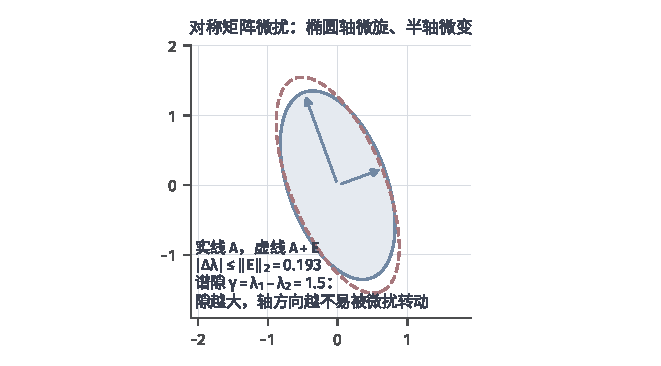
\includegraphics[width=112mm]{figures/00-shared/mathematical-preliminaries-upper/02-linear-spaces/matplotlib/ls-perturbation-ellipse/ls-perturbation-ellipse.pdf}
 \caption{对称矩阵微扰的谱与方向。实线椭圆为$\bm A$（特征值$2$与$0.5$，主轴
 方向$20^\circ$），虚线为$\bm A+\bm E$（$\lVert\bm E\rVert_2\approx0.193$）：轴
 微旋、半轴微变。新特征值约$2.18$与$0.37$，偏移$0.18$、$0.13$均小于
 $\lVert\bm E\rVert_2$，符合Weyl界；未扰动的谱隙$\delta=\lambda_1-\lambda_2=1.5$越大，
 特征方向越不易被微扰转动。}
 \label{fig:ls-perturbation-ellipse}
\end{figure}

Courant--Fischer定理把每个特征值写成Rayleigh商的最小最大值，而扰动$\bm E$对Rayleigh商的影响不超过$\lVert\bm E\rVert_2$，由此得到下面的界。
\begin{theorem}[Weyl特征值扰动界]
\label{thm:ls-weyl-eigenvalue}
对实对称$\bm A,\bm E\in\mathbb R^{d\times d}$，$\widetilde{\bm A}=\bm A+\bm E$与$\bm A$按降序配对的特征值满足
\begin{equation}
\begin{gathered}
|\widetilde\lambda_k-\lambda_k|
 \leq\lVert\bm E\rVert_2\\
k=1,\dots,d.
\end{gathered}
\label{eq:matrix-analysis-weyl-eigenvalue-perturbation}
\end{equation}
\end{theorem}
\begin{proof}
$\bm E$对称，由Rayleigh--Ritz定理，它的Rayleigh商介于最小与最大特征值之间，而它们的绝对值不超过$\lVert\bm E\rVert_2$，所以$|\bm x^\top\bm E\bm x|\leq\lVert\bm E\rVert_2\lVert\bm x\rVert_2^2$。取$\mathcal V=\operatorname{span}\{\bm q_1,\ldots,\bm q_k\}$（$\bm A$的前$k$个特征向量），其中每个$\bm x$满足
\[
 \bm x^\top\widetilde{\bm A}\bm x=\bm x^\top\bm A\bm x+\bm x^\top\bm E\bm x\geq(\lambda_k-\lVert\bm E\rVert_2)\lVert\bm x\rVert_2^2 .
\]
由Courant--Fischer定理，$\widetilde\lambda_k$不小于$\widetilde{\bm A}$在任一$k$维子空间上Rayleigh商的最小值，故$\widetilde\lambda_k\geq\lambda_k-\lVert\bm E\rVert_2$。把$\bm A$看作$\widetilde{\bm A}$加扰动$-\bm E$，交换二者的角色得$\lambda_k\geq\widetilde\lambda_k-\lVert\bm E\rVert_2$。
\end{proof}

Weyl界不需要特征值彼此分开，单重与重复特征值都适用。若$\bm A$正定且$\bm E$对称，并有$\|\bm E\|_2<\lambda_{\min}(\bm A)$，则对所有$0\leq t\leq1$，
\[
 \lambda_{\min}(\bm A+t\bm E)\geq\lambda_{\min}(\bm A)-\|\bm E\|_2>0.
\]
因此整条扰动线段都保持正定。这一统一下界将在矩阵函数微分中用于确认求逆和对数的定义域。


非对称矩阵的特征值没有这样的保证。

设$\bm A=\bm V\bm\Lambda\bm V^{-1}$可对角化，$\mu$是$\bm A+\bm E$的特征值而不是$\bm A$的特征值，$\bm w$为对应的特征向量（必要时取复数）。由$(\bm A+\bm E)\bm w=\mu\bm w$，令$\bm y=\bm V^{-1}\bm w\neq\bm0$，得$(\bm\Lambda-\mu\bm I)\bm y=-\bm V^{-1}\bm E\bm V\bm y$。$\mu$不是$\bm A$的特征值，所以对角矩阵$\bm\Lambda-\mu\bm I$可逆，于是$\bm y=-(\bm\Lambda-\mu\bm I)^{-1}\bm V^{-1}\bm E\bm V\bm y$。两边取范数并除以$\lVert\bm y\rVert_2$，得$1\leq\lVert(\bm\Lambda-\mu\bm I)^{-1}\rVert_2\,\kappa_2(\bm V)\lVert\bm E\rVert_2$；而对角矩阵$(\bm\Lambda-\mu\bm I)^{-1}$的范数是$1/\min_k|\lambda_k-\mu|$，于是得到Bauer--Fike界
\[
 \min_k|\mu-\lambda_k|\leq\kappa_2(\bm V)\lVert\bm E\rVert_2 .
\]
特征向量越接近线性相关，$\kappa_2(\bm V)$越大，界越宽。对称情形$\bm V$可取正交矩阵，$\kappa_2(\bm V)=1$，界与Weyl界同量级。

不可对角化时情况更糟，特征值的移动可以远大于扰动本身。
\begin{example}[反例：特征值的移动远大于扰动]
\label{ex:ls-jordan-eigenvalue-sensitivity}
给定$\bm N=\left[\begin{smallmatrix}0&1\\0&0\end{smallmatrix}\right]$，它的特征值全为$0$。在左下角加入扰动$\varepsilon$，得
\[
\begin{gathered}
\bm N_\varepsilon=\begin{bmatrix}0&1\\\varepsilon&0\end{bmatrix}\\
p_{\bm N_\varepsilon}(z)=z^2-\varepsilon ,
\end{gathered}
\]
扰动的大小为$\lVert\bm N_\varepsilon-\bm N\rVert_2=|\varepsilon|$。$\varepsilon>0$时特征值为$\pm\sqrt\varepsilon$，移动量为$\sqrt\varepsilon$；例如$\varepsilon=10^{-10}$时特征值移动$10^{-5}$，是扰动的$10^5$倍。$\varepsilon<0$时特征值为$\pm\mathrm i\sqrt{|\varepsilon|}$，实特征值消失。结论：特征值的移动量是$O(\sqrt{|\varepsilon|})$而非$O(|\varepsilon|)$，不能由扰动的范数乘一个常数控制。
\end{example}
可见对非对称矩阵，特征值的敏感程度取决于矩阵的结构：可对角化时，移动量至多是扰动的$\kappa_2(\bm V)$倍；不可对角化时，移动量甚至不与扰动成正比。

\subsection{奇异值的扰动}

Weyl界也给出奇异值的稳定性。把$\bm A\in\mathbb R^{m\times d}$嵌入对称分块矩阵$\left[\begin{smallmatrix}\bm0&\bm A\\\bm A^\top&\bm0\end{smallmatrix}\right]$，由$\bm A\bm v_i=\sigma_i\bm u_i$、$\bm A^\top\bm u_i=\sigma_i\bm v_i$可直接验证对每个正奇异值，向量$(\bm u_i,\pm\bm v_i)$是它的特征向量，特征值为$\pm\sigma_i$，其余特征值为零；而$\bm E$嵌入后谱范数不变。对嵌入矩阵应用Weyl界，得
\begin{equation}
 |\widetilde\sigma_i-\sigma_i|\leq\lVert\bm E\rVert_2 .
 \label{eq:matrix-analysis-singular-value-perturbation}
\end{equation}
截断SVD的误差$\sigma_{k+1}$（定理~\ref{thm:ls-best-low-rank}）因而也只移动不超过$\lVert\bm E\rVert_2$。

\subsection{子空间距离与主角}
\label{sec:ls-subspace-sensitivity}

比较特征向量时先要确定比较什么。同一子空间的基可以旋转、变号，单个基向量的变化不能当作子空间误差；特征值重复时，特征空间内部怎么换基都不改变子空间。所以比较对象必须是子空间本身，需要一个与基的选取无关的度量。图~\ref{fig:ls-principal-angles-subspaces}从两条过原点的直线看起：两直线的夹角与方向向量的选取无关；把一条直线的单位方向向量投影到另一条上，投影不掉的部分长度为$\sin\theta$。

\begin{figure}[htbp]
 \centering
 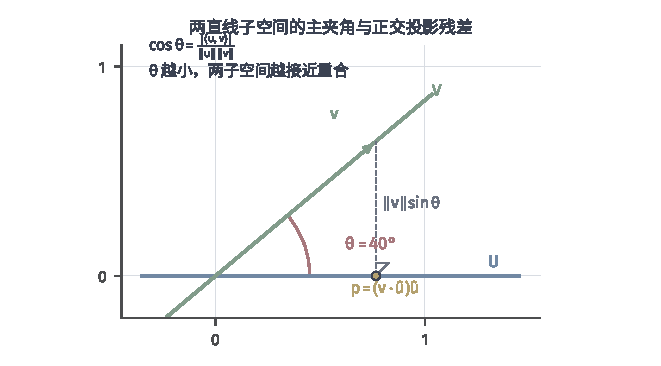
\includegraphics[width=112mm]{figures/00-shared/mathematical-preliminaries-upper/02-linear-spaces/matplotlib/ls-principal-angles-subspaces/ls-principal-angles-subspaces.pdf}
 \caption{两条直线子空间的主夹角。蓝线为$\bm U$、绿线为$\bm V$，红弧为主夹角
 $\theta=40^\circ$；黄点$\bm p$是$\bm v$在$\bm U$上的正交投影，灰虚线为投影
 垂线。$\cos40^\circ\approx0.766$、$\sin40^\circ\approx0.643$，残差长度
 $\lVert\bm v\rVert\sin\theta$即投影不掉的分量。}
 \label{fig:ls-principal-angles-subspaces}
\end{figure}

对一维子空间，若$\bm q,\widetilde{\bm q}$是单位方向向量，则$|\bm q^\top\widetilde{\bm q}|=\cos\theta$。高维子空间之间有多个夹角，由交叉内积矩阵的奇异值给出。
\begin{definition}[主夹角]
\label{def:matrix-analysis-principal-angles}
设$\bm Q,\widetilde{\bm Q}\in\mathbb R^{d\times r}$列标准正交，分别张成$r$维子空间。交叉矩阵$\bm Q^\top\widetilde{\bm Q}$的奇异值记为$\cos\theta_1\geq\dots\geq\cos\theta_r$，$0\leq\theta_1\leq\cdots\leq\theta_r\leq\pi/2$，这些$\theta_i$称为两个子空间的\term{主夹角}（principal angles）。
\end{definition}
这些奇异值都在$[0,1]$内，因为$\lVert\bm Q^\top\widetilde{\bm Q}\rVert_2\leq\lVert\bm Q\rVert_2\lVert\widetilde{\bm Q}\rVert_2=1$，所以$\theta_i$有定义。换基相当于把$\bm Q$、$\widetilde{\bm Q}$右乘正交矩阵，交叉矩阵的奇异值不变，所以主夹角只依赖子空间。

主夹角的正弦也可以直接读出。

设$\widetilde{\bm Q}_\perp$的列是$\widetilde{\bm Q}$列空间正交补的标准正交基。对单位向量$\bm a$，把$\bm Q\bm a$分解到$\widetilde{\bm Q}$的列空间与其正交补，由勾股定理，
\[
 \lVert\widetilde{\bm Q}^\top\bm Q\bm a\rVert_2^2+\lVert\widetilde{\bm Q}_\perp^\top\bm Q\bm a\rVert_2^2=\lVert\bm Q\bm a\rVert_2^2=1 .
\]
记$\bm C=\widetilde{\bm Q}^\top\bm Q$、$\bm X=\widetilde{\bm Q}_\perp^\top\bm Q$。上式对所有单位向量$\bm a$成立，说明对称矩阵$\bm X^\top\bm X$与$\bm I-\bm C^\top\bm C$的二次型处处相等，所以$\bm X^\top\bm X=\bm I-\bm C^\top\bm C$。$\bm C$是交叉矩阵的转置，奇异值为$\cos\theta_i$，所以$\bm X^\top\bm X$的特征值是$1-\cos^2\theta_i=\sin^2\theta_i$，即$\bm X$的奇异值是$\sin\theta_i$。

子空间的误差还可以用正交投影$\bm P=\bm Q\bm Q^\top$、$\widetilde{\bm P}=\widetilde{\bm Q}\widetilde{\bm Q}^\top$之差表示，它与基的选取无关。可以证明
\[
 \begin{gathered}
\lVert\bm P-\widetilde{\bm P}\rVert_2=\sin\theta_r\\
\tfrac12\lVert\bm P-\widetilde{\bm P}\rVert_{\mathrm F}^2=\sum_{i=1}^r\sin^2\theta_i .
 \end{gathered}
\]
第二式可以直接验证：由$\operatorname{tr}\bm P=\operatorname{tr}\widetilde{\bm P}=r$与$\operatorname{tr}(\bm P\widetilde{\bm P})=\lVert\bm Q^\top\widetilde{\bm Q}\rVert_{\mathrm F}^2=\sum_i\cos^2\theta_i$，得$\lVert\bm P-\widetilde{\bm P}\rVert_{\mathrm F}^2=2r-2\sum_i\cos^2\theta_i=2\sum_i\sin^2\theta_i$。第一式说明投影矩阵之差的谱范数就是最大主夹角的正弦，它的证明较长，这里从略。

\subsection{特征子空间的扰动}

有了主夹角，就可以估计扰动使特征子空间转过多大的角度。

设$\bm A$、$\widetilde{\bm A}=\bm A+\bm E$实对称，$\bm Q$的列是$\bm A$的前$k$个单位特征向量，$\widetilde{\bm Q}$的列是$\widetilde{\bm A}$的前$k$个单位特征向量。要求目标特征值与扰动后其余特征值之间有间隔
\[
 \gamma=\lambda_k-\widetilde\lambda_{k+1}>0 .
\]
记$\widetilde{\bm Q}_\perp$为$\widetilde{\bm A}$其余特征向量组成的矩阵，$\widetilde{\bm\Lambda}_2$为对应的特征值对角矩阵，$\bm\Lambda_1=\operatorname{diag}(\lambda_1,\ldots,\lambda_k)$，并令$\bm X=\widetilde{\bm Q}_\perp^\top\bm Q$。由上一小节，它的奇异值就是两个子空间主夹角的正弦。

把$\widetilde{\bm Q}_\perp^\top\widetilde{\bm A}=\widetilde{\bm\Lambda}_2\widetilde{\bm Q}_\perp^\top$右乘$\bm Q$，把$\bm A\bm Q=\bm Q\bm\Lambda_1$左乘$\widetilde{\bm Q}_\perp^\top$，两式相减，由$\widetilde{\bm A}-\bm A=\bm E$得
\[
 \widetilde{\bm\Lambda}_2\bm X-\bm X\bm\Lambda_1=\widetilde{\bm Q}_\perp^\top\bm E\bm Q .
\]
这是关于$\bm X$的线性方程，两侧的系数矩阵都是对角的，因此可以逐元素求解（第~\ref{chap:linear-equations-and-optimization}章把形如$\bm A\bm X+\bm X\bm B=\bm C$的方程称为Sylvester方程）。逐元素写出为$(\widetilde\lambda_j-\lambda_i)X_{j,i}=(\widetilde{\bm Q}_\perp^\top\bm E\bm Q)_{j,i}$，其中$i\leq k<j$。由降序，$\lambda_i-\widetilde\lambda_j\geq\lambda_k-\widetilde\lambda_{k+1}=\gamma$，逐元素相除得
\[
 \lVert\bm X\rVert_{\mathrm F}\leq\frac{\lVert\widetilde{\bm Q}_\perp^\top\bm E\bm Q\rVert_{\mathrm F}}{\gamma}\leq\frac{\lVert\bm E\bm Q\rVert_{\mathrm F}}{\gamma}.
\]
左端的平方是主夹角正弦的平方和，所以这个平方和由扰动与谱隙之比控制。更细的论证给出谱范数下的同型结论，称为Davis--Kahan谱隙界\scite{math-golub2013matrix}：
\begin{equation}
 \lVert\widetilde{\bm P}-\bm P\rVert_2=\sin\theta_{k}
 \leq\frac{\lVert\bm E\rVert_2}{\gamma}.
 \label{eq:matrix-analysis-eigenvector-gap-bound}
\end{equation}
$\gamma$用到扰动后的特征值。若只知道未扰动的谱隙$\delta=\lambda_k-\lambda_{k+1}$，由Weyl界$\widetilde\lambda_{k+1}\leq\lambda_{k+1}+\lVert\bm E\rVert_2$，得$\gamma\geq\delta-\lVert\bm E\rVert_2$；当$\lVert\bm E\rVert_2\leq\delta/2$时，$\gamma\geq\delta/2$，右端不超过$2\lVert\bm E\rVert_2/\delta$。

谱隙在分母上：谱隙越小，子空间越容易被扰动转动。下面的二维例子可以精确算出转角。
\begin{example}[谱隙与特征方向的转角]
\label{ex:ls-gap-direction-rotation}
给定$\bm A_\alpha=\operatorname{diag}(\alpha,-\alpha)$（$\alpha>0$）与交叉扰动$\bm E=\varepsilon\left[\begin{smallmatrix}0&1\\1&0\end{smallmatrix}\right]$（$\varepsilon>0$）。$\bm A_\alpha$的两个特征值相距$2\alpha$，最大特征方向是$\bm e_1$。记$r=\sqrt{\alpha^2+\varepsilon^2}$，取$\theta\in(0,\pi/4)$满足$\cos2\theta=\alpha/r$、$\sin2\theta=\varepsilon/r$，即$\theta=\tfrac12\arctan(\varepsilon/\alpha)$。扰动后的矩阵可以写成
\[
 \bm A_\alpha+\bm E=\begin{bmatrix}\alpha&\varepsilon\\\varepsilon&-\alpha\end{bmatrix}
 =r\begin{bmatrix}\cos2\theta&\sin2\theta\\\sin2\theta&-\cos2\theta\end{bmatrix}.
\]
由两角差公式，
\[
 (\bm A_\alpha+\bm E)\begin{bmatrix}\cos\theta\\\sin\theta\end{bmatrix}
 =r\begin{bmatrix}\cos(2\theta-\theta)\\\sin(2\theta-\theta)\end{bmatrix}
 =r\begin{bmatrix}\cos\theta\\\sin\theta\end{bmatrix},
\]
而迹为零，另一个特征值是$-r$。所以最大特征方向从$\bm e_1$转到$(\cos\theta,\sin\theta)^\top$，转角为
\[
 \theta=\tfrac12\arctan\frac{\varepsilon}{\alpha}\approx\frac{\varepsilon}{2\alpha}\qquad(\varepsilon\ll\alpha).
\]
与界~\eqref{eq:matrix-analysis-eigenvector-gap-bound}比较：$\lVert\bm E\rVert_2=\varepsilon$，$\gamma=\lambda_1-\widetilde\lambda_2=\alpha+r\approx2\alpha$，界给出$\sin\theta\leq\varepsilon/\gamma\approx\varepsilon/(2\alpha)$，与实际转角同阶。结论：转角近似与谱隙$2\alpha$成反比，$\alpha$减半，转角加倍。
\end{example}
图~\ref{fig:matrix-analysis-gap-direction}画出这一关系。

谱隙只需存在于目标特征值组与组外之间，组内的特征值不必彼此分开。例如在$\operatorname{diag}(2,2,0)$中，特征值$2$对应的平面内每个单位向量都是特征方向，单独比较某个向量没有意义。但取$k=2$，未扰动的谱隙为$\delta=2-0=2$，由上面的推论，$\lVert\bm E\rVert_2\leq1$时整个二维特征子空间的最大主夹角满足$\sin\theta_2\leq2\lVert\bm E\rVert_2/\delta=\lVert\bm E\rVert_2$。

奇异子空间也有同样的结论。对第~\ref{sec:ls-spectral-value-sensitivity}节的对称嵌入矩阵$\left[\begin{smallmatrix}\bm0&\bm A\\\bm A^\top&\bm0\end{smallmatrix}\right]$作同样的谱隙论证，可知奇异子空间的稳定性由截断处的间隔$\sigma_k-\sigma_{k+1}$控制。所以截断SVD的误差$\sigma_{k+1}$总是稳定的，它所用的主方向却只在截断处有间隔时才稳定。

\begin{figure}
 \centering
 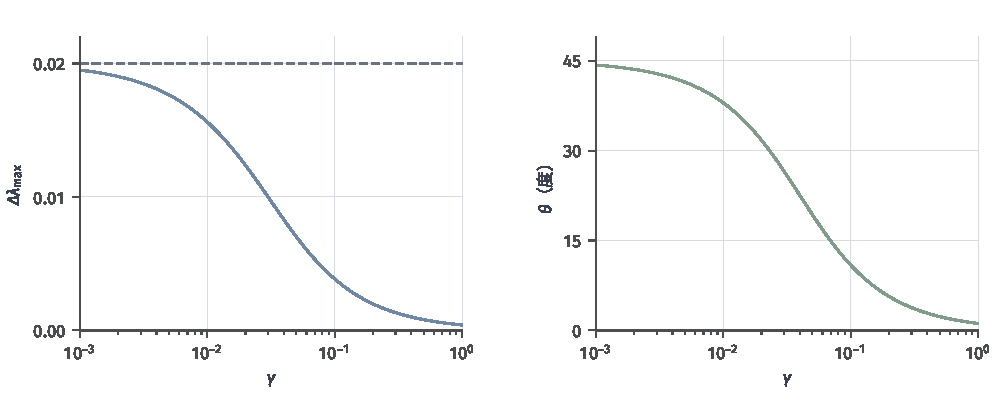
\includegraphics[width=0.92\linewidth]{figures/00-shared/mathematical-preliminaries-upper/02-linear-spaces/matplotlib/matrix-analysis-gap-direction/figure.pdf}
 \caption{谱隙方向示意：$\bm A_\alpha$的两个特征值相距$2\alpha$（谱隙），
 交叉扰动$\varepsilon$把最大特征方向转过约$\varepsilon/(2\alpha)$；
 谱隙越小，同样扰动转过的角度越大。}
 \label{fig:matrix-analysis-gap-direction}
\end{figure}

本节得到的结论是：把矩阵本身当作输入时，对称矩阵的特征值与任意矩阵的奇异值都是良态的，移动不超过$\lVert\bm E\rVert_2$，不要求特征值彼此分开；特征子空间要用与基无关的主夹角比较，它的转角由扰动与谱隙之比控制，谱隙越小越容易被转动；非对称矩阵的特征值可能对扰动非常敏感，敏感程度由特征向量矩阵的条件数或不可对角化的结构决定。条件数与谱的扰动讨论的都是一次作用或一次分解。下一节转向同一个矩阵的反复作用。
